\documentclass{jfsma}
\usepackage{lmodern}
\usepackage{hyperref}
\usepackage{caption}
\usepackage{cuted}
\usepackage{etoolbox}

\titre{Automatic Observer For Real-Time Strategy Games} % On garde ce titre ?
\auteur{Emmanuel \textsc{Hadoux}}{emmanuel.hadoux@gmail.com}
\auteur{Thomas \textsc{Huraux}}{thomas.huraux@gmail.com}
\institution{
  LIP6, CNRS UMR 7606,\\
  Universit\'e Pierre et Marie Curie, France}

\begin{document}
	\maketitle
	
	\begin{strip}
  \centering\noindent
  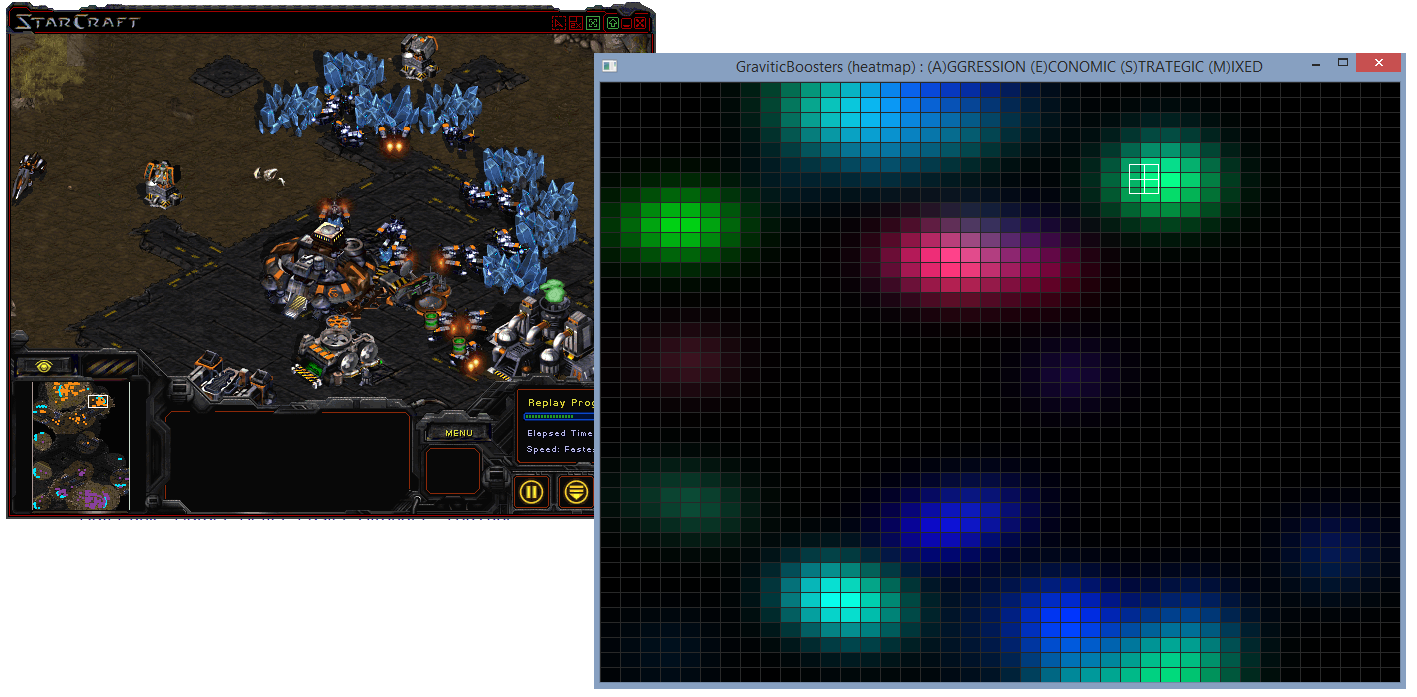
\includegraphics[scale=0.35]{gfx/GB}
\end{strip}

	\section{Introduction}
    	Electronic sport (\textit{e-sport}) is a not-so-young discipline slowly growing in western countries.
        It takes root in South-Korea about 15 years ago. 
        In this country, players are rockstars, brawling in front of ten of thousands viewers, on site or on national TV. % T : ca c'est un peu de la branlette
        The first game entering the closed category of e-sport was Starcraft 1. % T: faut voir si on parle tout de suite de SC ou alors on vise un truc plus générique
        This fast-paced real-time strategy game (\textit{RTS}) was released in 1998.
        
        During battles between the two armies, players can reach picks of 300 actions-per-minutes (\textit{APM}).
        For obvious related reasons, viewers cannot follow the game by watching the screens of the players.
        Competitions thus require an external observer following the game and showing important actions.
        However, being an observer requires a comprehensive knowledge of the game as well as anticipation and entertainment faculties. 
        Few persons are able to gather all those skills, making them even more famous than some professional players.
        
        \medskip
        In this work, we propose to replace the human observer by an automatic observer, able to catch every piece of action.
        etc.
        
\section{Overview}
We develop an automatic observer called \emph{Gravitic Boosters}...

Each entity of the has three potentials calculated in real time during the game:
\begin{description}
\item[aggressive potential]
\item[economic potential]
\item[strategic potential]
\end{description}

The map is then discretized so that each cell aggregates the potential of all entities that compose it.

To better position the camera on the action, we smooth the potential matrix with a gaussian kernel. This allows in particular to position the camera between two armies facing each other.
        
\section{Conclusion}
...
\end{document}